\section{Composite}

Esse padrão fornece uma estrutura de objetos 
organizados como uma árvore, representados 
por uma hierarquia parte-todo. 
Ele torna possível tratar tanto o conjunto 
quanto os objetos individuais de forma 
uniforme, sem que seja necessário conhecer 
os elementos pertencentes a um conjunto para 
tratá-lo.\cite{gamma:1995}

A figura \ref{composite_struct} demonstra a 
estrutura do padrão, onde uma interface Component 
define tanto um objeto nó, representado pela 
classe Composite, quanto um objeto folha, 
representado pela classe Leaf. Os elementos 
filhos da classe Composite são todos instâncias 
de Component, o que faz com que a classe não 
saiba se seus filhos são outros objetos compostos 
ou se são objetos folha.

\begin{figure}[htb]
	\caption{\label{composite_struct}Estrutura do Composite}
	\begin{center}
	    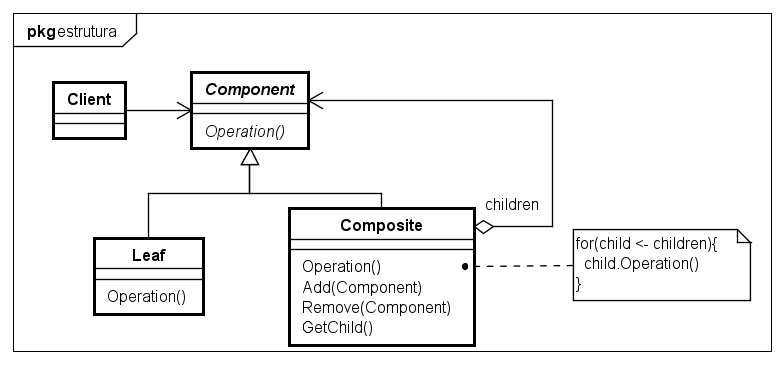
\includegraphics[scale=0.5]{5_padroes-contexto-funcional/5.2_estruturais/5.2.3_composite/composite_estrutura.png}
	\end{center}
\end{figure}

\subsection*{Exemplo Orientado a Objetos}

Como exemplo, é apresentada uma ferramenta gráfica 
onde o usuário pode agrupar diversas formas e 
elementos 
para formar diagramas maiores e mais complexos. 
Apesar do usuário tratar esses diagramas como um 
único elemento gráfico, a aplicação precisa levar 
em consideração todos os elementos dos quais eles 
são compostos. O padrão Composite permite 
abstrair os elementos menores, tratando o elemento 
composto como algo único, da mesma forma que 
são tratados os elementos não compostos. A figura 
\ref{composite_exemplo} demonstra o diagrama de 
classes para esse exemplo, enquanto o código 
\ref{oocomposite} traz um exemplo de implementação.

\begin{figure}[htb]
	\caption{\label{composite_exemplo}Exemplo de Composite}
	\begin{center}
	    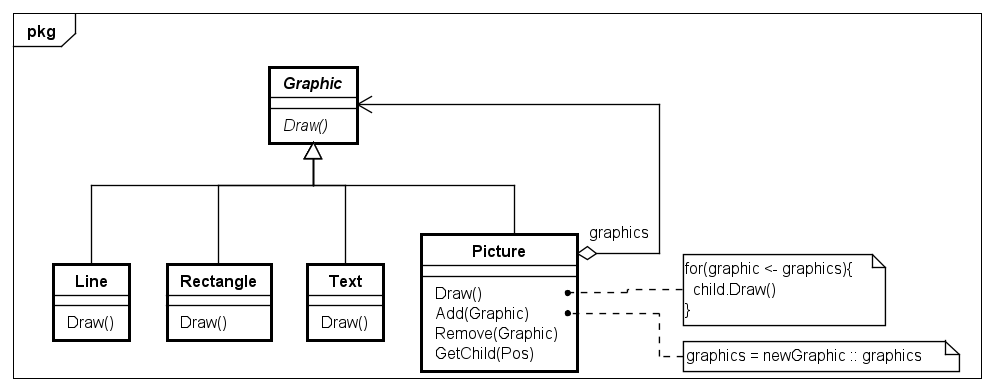
\includegraphics[scale=0.5]{5_padroes-contexto-funcional/5.2_estruturais/5.2.3_composite/composite_exemplo.png}
	\end{center}
\end{figure}

\begin{lstlisting}[caption={Composite Orientado a Objetos},label=oocomposite]

trait Graphic {
  def Draw();
}

class Picture extends Graphic {
  private var graphics : List[Graphic] = List()

  def Draw() : Unit = {
    graphics.foreach(f => f.Draw())
  }

  def Add(graphic: Graphic): Unit = {
    graphics = graphic :: graphics
  }

  def Remove(graphic: Graphic) : Unit = {
    graphics = graphics.filter(g => g != graphic)
  }

  def GetChild(pos : Int) : Graphic = graphics(pos)
}

class Text extends Graphic {
  def Draw() : Unit = {
    //Desenha o elemento na tela
  }
}

class Rectangle extends Graphic {
  def Draw() : Unit = {
    //Desenha o elemento na tela
  }
}

class Line extends Graphic {
  def Draw() : Unit = {
    //Desenha o elemento na tela
  }
}

\end{lstlisting}

\subsection*{Contexto Funcional}

O código \ref{fpcomposite} demonstra como é 
possível declarar a estrutura do padrão Composite 
utilizando funções de alta ordem. A função 
Draw, definida na linha 2, é equivalente à função 
Draw da classe Picture do exemplo orientado a 
objetos. A diferença é que ela recebe como parâmetro 
uma lista de funções e retorna uma nova função, 
com a mesma assinatura, que executa todas as 
funções da lista. As funções DrawLine, DrawRectangle 
e DrawText, definidas nas linhas 5, 10 e 15, 
respectivamente, são equivalentes aos elementos 
folha da estrutura de árvore proposta pelo 
Composite. Elas recebem como parâmetro todos 
os valores necessários para desenhar os elementos 
gráficos e retornam uma função para 
desenhá-los.

As funções retornadas são adicionadas a uma 
lista que deve ser passada para a função Draw. 
Como a assinatura de Draw é igual à das funções 
que ela recebe, uma nova chamada de Draw pode 
conter tanto "funções folha" quanto funções 
que são resultado da chamada de Draw. Isso 
favorece a vantagem do padrão Composite de 
permitir que toda a estrutura seja tratada 
de forma indefinida, sem que a função 
cliente precise saber se está tratando de um 
grupo de elementos ou de um elemento apenas. 

\begin{lstlisting}[caption={Composite Funcional},label=fpcomposite]
    
def Draw(functions : List[() => Unit]) : () => Unit =
  () => functions.foreach((function) => function())

def DrawLine(length : Int) : () => Unit =
  () => {
    // Desenha linha
  }

def DrawRectangle(width : Int, height : Int) : () => Unit =
  () => {
    // Desenha retângulo
  }

def DrawText(text : String) : () => Unit =
  () => {
    // Escreve texto
  }
    
\end{lstlisting}

O código \ref{fpcompositeapp} demonstra a 
aplicação do padrão. O valor DrawGraphics, 
definido na linha 2, é o resultado da aplicação 
de Draw para uma lista contendo uma função que 
desenha uma linha e uma função que desenha 
um retângulo. Já o valor DrawAllText, definido 
na linha 7, é definida através de duas funções 
que desenham texto. Na linha 12, o valor 
DrawEverything é definido a partir das funções 
armazenadas nos valores DrawGraphics e 
DrawAllText. Ao ser executado, ele executará 
também todas as funções definidas anteriormente 
tratando todo o conjunto como um único elemento, 
da forma como o padrão Composite propõe.

\begin{lstlisting}[caption={Aplicação do Composite Funcional},label=fpcompositeapp]
    
val DrawGraphics : () => Unit = Draw(
  List(
    DrawLine(5),
    DrawRectangle(4, 5)))

val DrawAllText : () => Unit = Draw(
  List(
    DrawText("Text 1"),
    DrawText("Text 2")))

val DrawEverything : () => Unit = Draw(
  List(
    DrawGraphics,
    DrawAllText))
    
\end{lstlisting}